% !TEX encoding = UTF-8
% !TEX TS-program = pdflatex
% !TEX root = ../Tesi.tex
% !TEX spellcheck = it-IT

%************************************************
\chapter{Velocity Obstacle}
\label{cap:vo}
%************************************************

Velocity Obstacle \'e un algoritmo di local Collision Avoidance di navigazione tra altri robot e ostacoli statici o dinamici nello stesso ambiente.
\\In due dimensione \'e definito come segue.

\section{Velocity Obstacle}

{\bfseries\textit{A}} rappresenta un robot e {\bfseries\textit{B}} rappresenta un ostacolo dinamico (altro robot) nel piano,
{\bfseries\textit{p}\ped A} e {\bfseries\textit{p}\ped B} rappresentano le posizioni correnti di {\bfseries\textit{A}} e di {\bfseries\textit{B}}, rispettivamente,  {\bfseries\textit{v}\ped A} e {\bfseries\textit{v}\ped B} rappresentano le loro velocit\'a correnti.


\subsection{Collision Cone}

Noi definiamo \textit{Collision Cone},  \textit{CC}\ped {A,B}, l'insieme delle \textit{colliding relative velocities} tra {\bfseries\textit{A'}} e {\bfseries\textit{B'}}:
\begin{gather}
CC_{A,B} = \{ \boldsymbol{v}_{A,B} | \lambda_{A,B} \cap \boldsymbol{B'} \neq \oslash \}
\end{gather}
dove  {\bfseries\textit{v}\ped {A,B}} rappresenta la velocit\'a relativa di {\bfseries\textit{A'}} rispetto {\bfseries\textit{B'}}, {\bfseries\textit{v}\ped {A,B}} = {\bfseries\textit{v}\ped A} - {\bfseries\textit{v}\ped B}, e $\lambda\ped {A,B}$  \'e la linea di {\bfseries\textit{v}\ped {A,B}}.
\\Questo cono \'e la parte di piano delimitata da tue tangenti, $\lambda\ped f$ e $\lambda\ped r$, con apice in {\bfseries\textit{A'}}. Ogni velocit\'a relativa all'interno delle due tangenti rappresenta una collisione tra i due robot. 
Per considerare multipli ostacoli, \'e utile stabilire delle condizioni equivalenti sulle velocit\'a assolute di {\bfseries\textit{A}}. Questo \'e fatto semplicemente sommando la velocit\'a di {\bfseries\textit{B}}, {\bfseries\textit{v}\ped B}, per ogni velocit\'a nel \textit{CC}\ped {A,B} o, equivalentemente, traslando il cono delle collisioni \textit{CC}\ped {A,B} di {\bfseries\textit{v}\ped B}. Definendo \textit{Velocity Obstacle VO} come:
\begin{gather}
VO= CC_{A,B} \oplus \boldsymbol{v}_{B} 
\end{gather}
dove $\oplus$ \'e l' operatore somma vettoriale di Minkowski.

\subsection{Time horizon}
Siccome VO \'e basato su una approssimazione lineare della traiettoria degli ostacoli, usando questo per predirre delle collisioni remote, potrebbe essere poco accurato se gli ostacoli non si muovono in linea retta. \\Noi definiamo \textit{collisione imminente}, tra robot e ostacolo, se succeder\'a in un tempo \textit{t}<\textit{T}\ped h, dove \textit{T}\ped h \'e un determinato spazio temporale chiamato \textit{time horizon}, selezionato in base al sistema dinamico, alla traiettoria dell'ostacolo e dalla computazione delle manovre per schivare l'ostacolo.
\\Avendo individuato una collisione imminete, noi modifichiamo l'insieme \textit{VO} sottraedo da esso l'insieme del \textit{VO}\ped h definito come segue:
\begin{gather}
VO_h=  \{ \boldsymbol{v}_{A} | \boldsymbol{v}_{A} \in VO, norm( \boldsymbol{v}_{A,B})\leq \tfrac{d_m}{T_h} \}
\end{gather}
dove \textit{d}\ped m \'e la pi\'u piccola distanza tra il robot e l'ostacolo. L'insieme \textit{VO}\ped h rappresenta le velocit\'a che risultano essere in collisione se prese al di sopra del time horizon.
\begin{figure}
\centering 
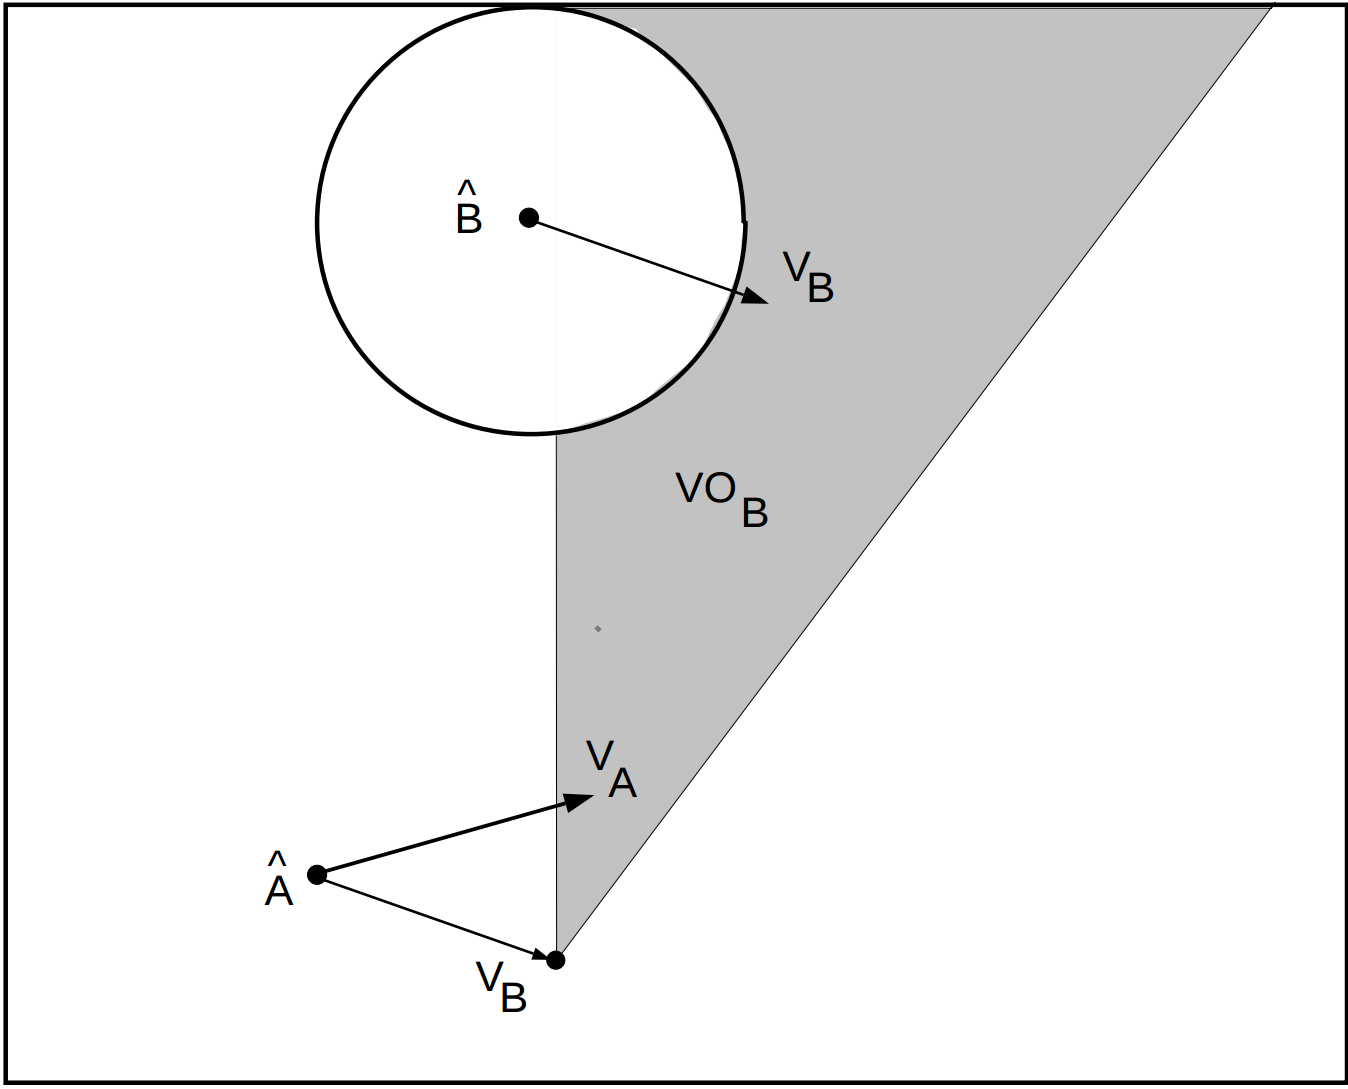
\includegraphics[width=0.6\columnwidth]{vo} 
\caption[Velocity Obstacle traslato della velocit\'a di B]{Velocity Obstacle traslato della velocit\'a di B}
\label{fig:vo} 
\end{figure}

\subsection{New velocity}
La computazione della nuova velocit\'a, in ogni time-step, deve essere selezionata fuori dal VO.
 Sfortunatamente, il concetto di Velocity Obstacle porta alla creazione di traiettorie oscillatorie sgradevoli.
 \\Pi\'u precisamente, se i robot \textit{A} e \textit{B} si stanno muovendo, rispettivamente, con {\bfseries\textit{v}\ped A} e {\bfseries\textit{v}\ped B}, si avr\'a che {\bfseries\textit{v}\ped A} $\in$ {\textit{VO}\ped {A,B}}({\bfseries\textit{v}\ped B}) e {\bfseries\textit{v}\ped B} $\in$ {\textit{VO}\ped {B,A}}( {\bfseries\textit{v}\ped A}).
 Quindi, lungo le stesse velocit\'a correnti, saranno in collisione. Perci\'o l'agente \textit{A} decider\'a di modificare la sua velocit\'a con {\bfseries\textit{v'}\ped A}, tale che sia fuori dal Velocity Obstacle di \textit{B}. Allo stesso tempo, \textit{B} modificher\'a la sua velocit\'a {\bfseries\textit{v'}\ped B}, che dovr\'a essere scelta fuori dal Velocity Obstacle di \textit{A}.
 \\Quindi, in questa nuova situazione, le vecchie velocit\'a {\bfseries\textit{v}\ped A} e {\bfseries\textit{v}\ped B} saranno fuori dal Velocity Obslacle di \textit{B} e \textit{A}, rispettivamente  {\bfseries\textit{v}\ped A} $\notin$ {\textit{VO}\ped {A,B}}({\bfseries\textit{v'}\ped B}) e  {\bfseries\textit{v}\ped B} $\notin$ {\textit{VO}\ped {B,A}}({\bfseries\textit{v'}\ped A}).
 Se entrambi gli agenti preferiscono le vecchie velocit\'a, per esempio perch\'e li porta direttamente al proprio \textit{goal}, le sceglieranno ancora. Nel ciclo successivo, queste velocit\'a si tradurranno in una collisione e loro (A e B) probabilmente sceglieranno di nuovo {\bfseries\textit{v'}\ped A} e {\bfseries\textit{v'}\ped B}, e cos\'i via.
\\Perci\'o gli agenti oscillano tra queste due velocit\'a, creando una traiettoria oscillatoria.

%%%%%%%%%%%%%%%%%%%%%%%%%%%%%%%%%%%%%%%%%%%%%%%%%%%%%%%%%%%%
